\themaN
\graphicspath{{../Ch17_Multiplications/Images/}}

\chapter{La multiplication}
\label{C14}


%%%%%%%%%%%%%%%%%%%%%%%%%%%%%%%%%%
%%%%%%%%%%%%%%%%%%%%%%%%%%%%%%%%%%
\begin{prerequis}[Connaissances et compétences abordées]
   \begin{itemize}
      \item Connaître des propriétés de la multiplication, et notamment la commutativité et la distributivité simple.
      \item Dans un calcul en ligne, utiliser des parenthèses pour indiquer ou respecter une chronologie dans les calculs.
      \item Connaître et mettre en œuvre un algorithme de calcul posé pour effectuer la multiplication de nombres entiers ou décimaux.
   \end{itemize}
\end{prerequis}

\vfill

\begin{debat}[Débat : multiplication par 9] 
   On peut facilement retrouver le résultat de la \og table des 9 \fg{} avec\dots{} une paire de main ! \\
   Par exemple, calculons $8\times9$ :
   \begin{itemize}
      \item placer les faces des mains devant soi, abaisser le 8\up{e} doigt en partant de la gauche ;
      \item les doigts à gauche du doigt abaissé correspondent au nombre de dizaines ;
      \item les doigts à droite du doigt abaissé correspondent au nombre d'unités.
   \end{itemize}
   Ici, $8\times9 =72$. \\ [1mm]
   Cette technique fonctionne pour la multiplication par 9 d'un nombre entier compris entre 1 et 10 inclus.
   \begin{center}
      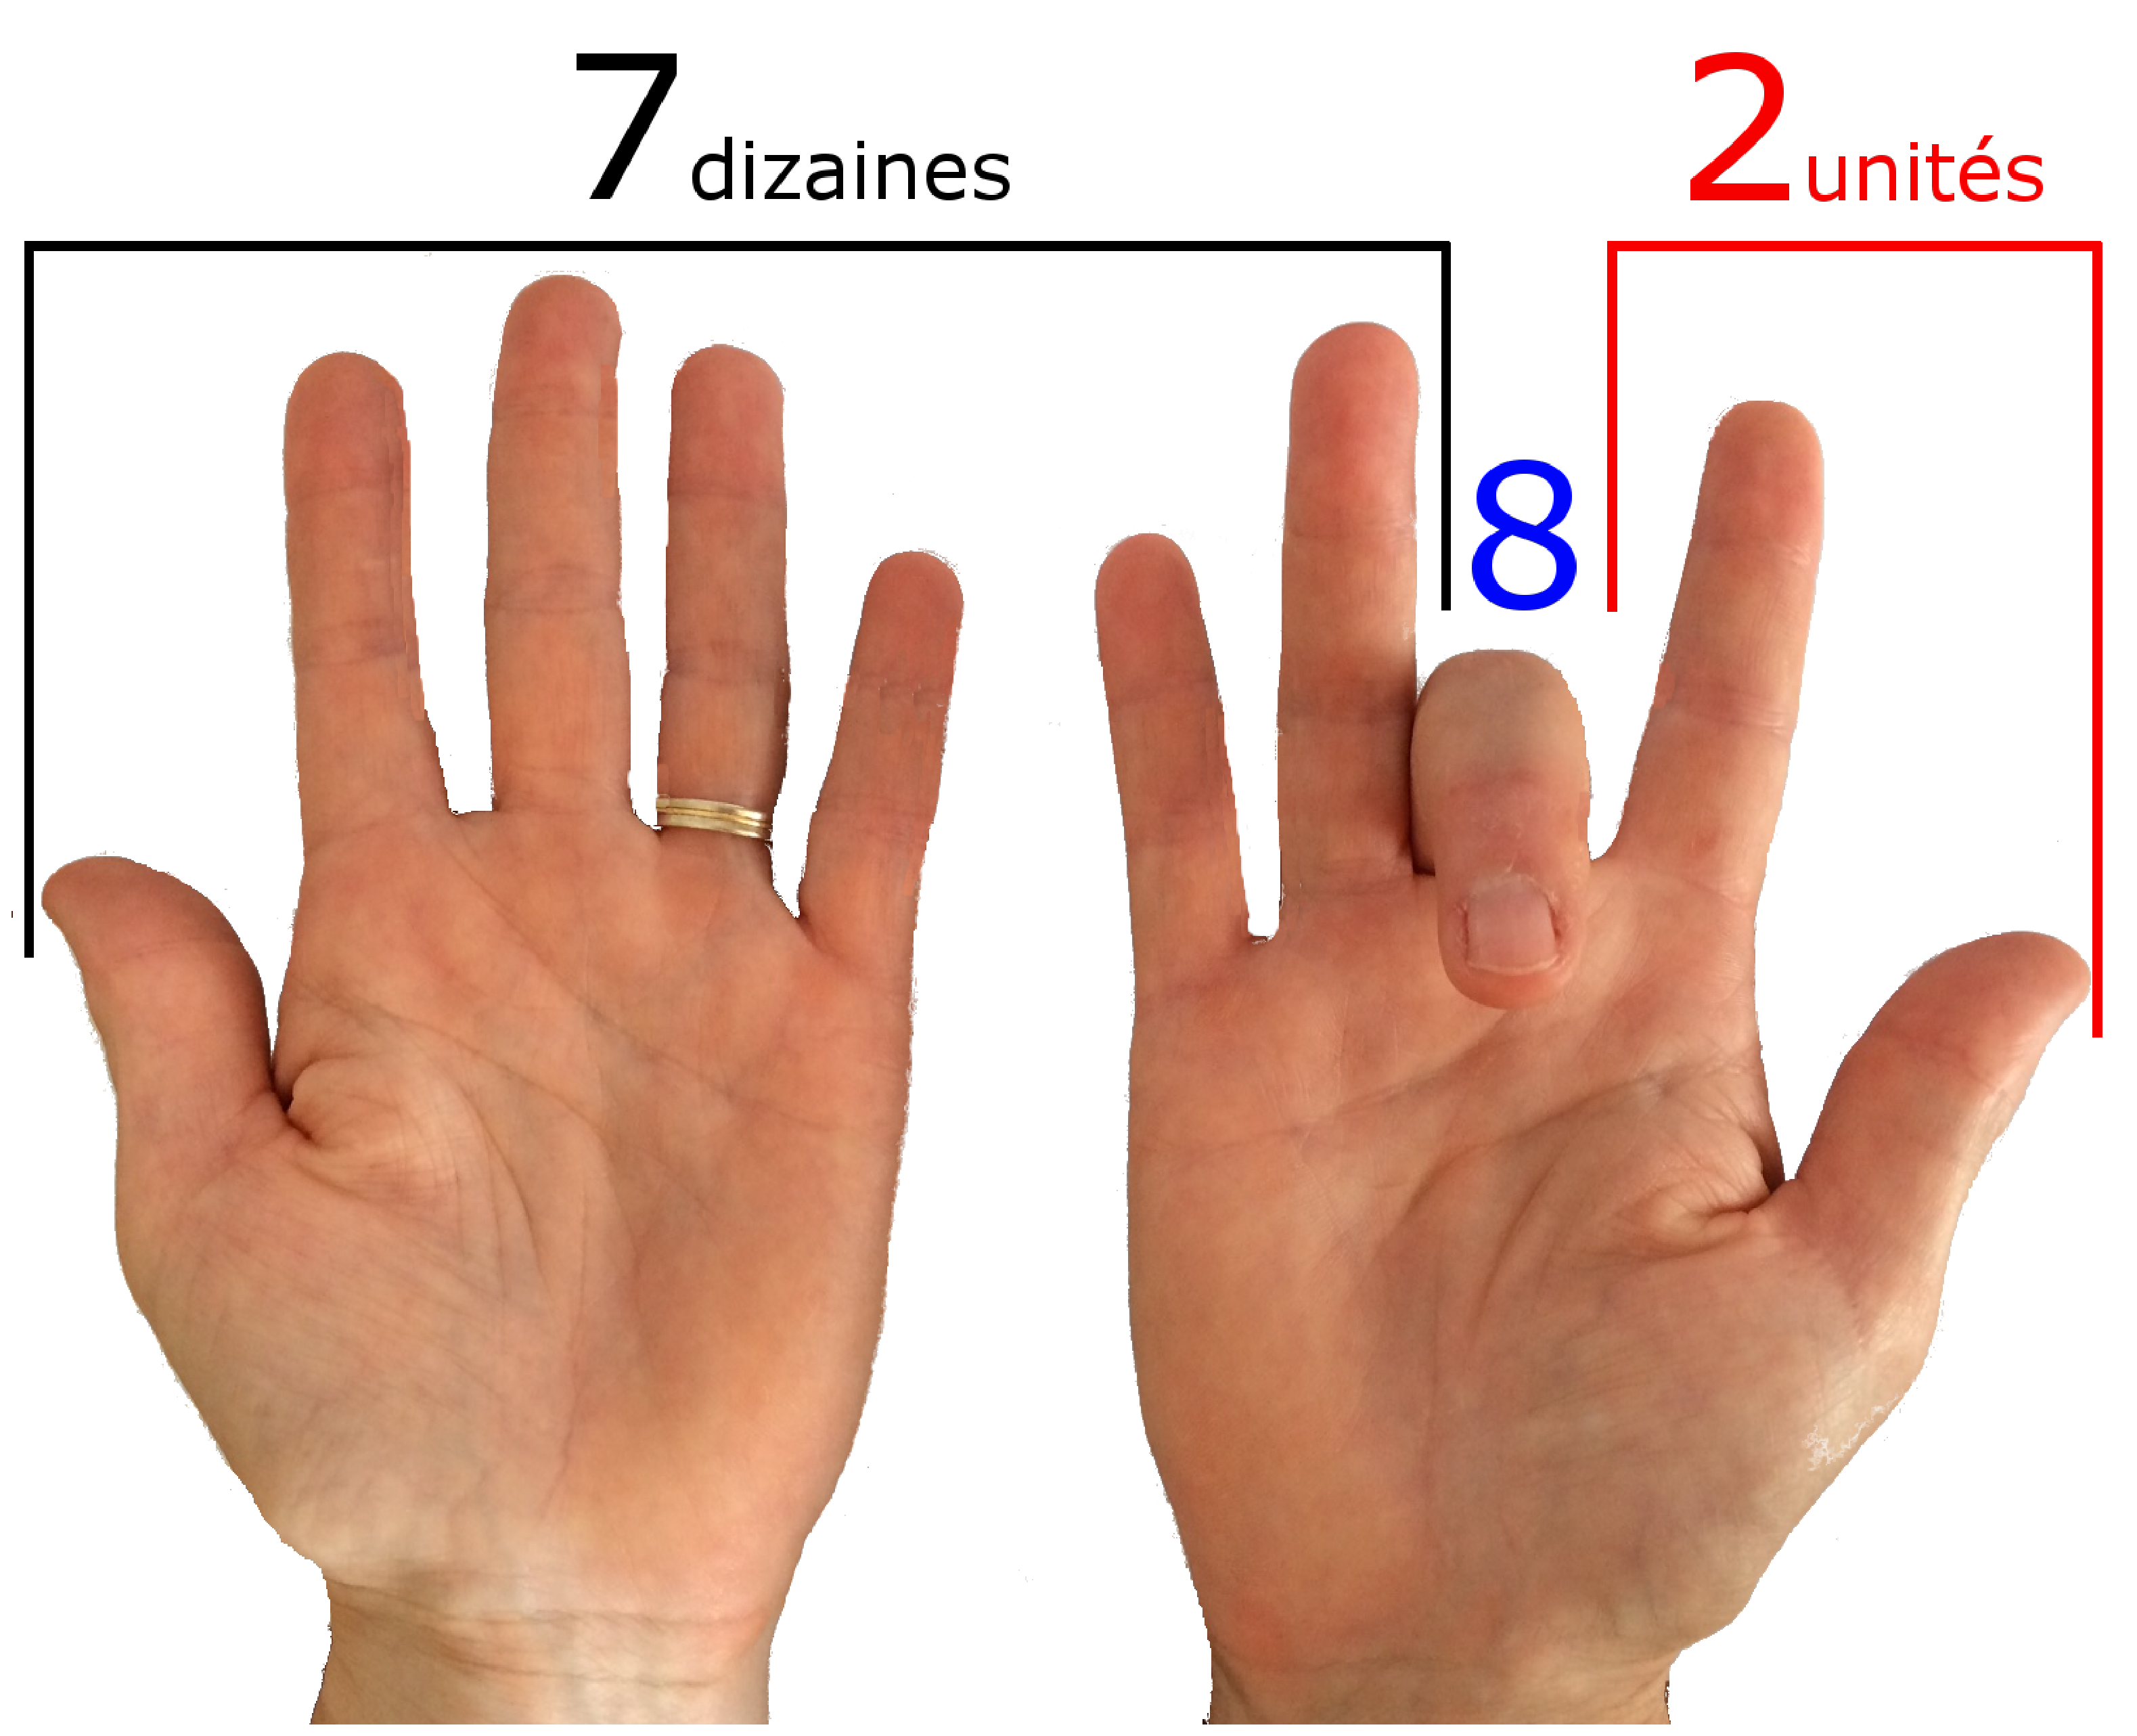
\includegraphics[width=5cm]{mains}
   \end{center}
   \bigskip
   \begin{cadre}[B2][F4]
      \begin{center}
         Vidéo : \href{https://www.youtube.com/watch?v=BPL7gmfH7V8}{\bf Table de multiplication avec les doigts}, chaîne YouTube {\it Les Parents Créatifs}.
      \end{center}
   \end{cadre}
\end{debat}

\vfill

\textcolor{PartieGeometrie}{\large\sffamily\bfseries Cahier de compétences} : chapitre 2, exercices 16 à 43 ; 59 à 61 ; 64.


%%%%%%%%%%%%%%%%%%%%%%%%%%%%%%%%%%%%
%%%%%%%%%%%%%%%%%%%%%%%%%%%%%%%%%%%%%
\activites

\begin{activite}[Les multiplications incomplètes]
   {\bf Objectifs} : calculer une multiplication ; résoudre un problème de calcul mental ; compléter un tableau à double entrée.
   \begin{QCM}
   Compléter ces tables de multiplication dont on a effacé le contenu de certaines cases. Les nombres sont tous strictement positifs, il ne peut pas y avoir deux fois le même nombre sur une même colonne ou une même ligne. \medskip
   {\hautab{1.8}
   \partie[piste verte] \medskip
      \hfill
      \begin{tabular}{|C{0.5}||C{0.5}|C{0.5}|}
         \hline
         {\Large $\times$} & & \\
         \hline\hline
         & & 24 \\
         \hline
         & 25 & 30 \\
         \hline
      \end{tabular}
      \hfill
      \begin{tabular}{|C{0.5}||C{0.5}|C{0.5}|}
         \hline
         {\Large $\times$} & & 7 \\
         \hline\hline
         & & 21 \\
         \hline
         4 & 8 & \\
         \hline
      \end{tabular}
      \hfill
      \begin{tabular}{|C{0.5}||C{0.5}|C{0.5}|}
         \hline
         {\Large $\times$} & 6 & \\
         \hline\hline
         & 24 & 32 \\
         \hline
         & 36 & \\
         \hline
      \end{tabular}
      \hfill
      \begin{tabular}{|C{0.5}||C{0.5}|C{0.5}|}
         \hline
         {\Large $\times$} & 3 & \\
         \hline\hline
         & & 18 \\
         \hline
         5 & & 45 \\
         \hline
      \end{tabular}
      \hspace*{1cm} \\
         
   \partie[piste bleue] \medskip
      \hfill
      \begin{tabular}{|C{0.5}||C{0.5}|C{0.5}|C{0.5}|}
         \hline
         {\Large $\times$} & 2 & & \\
         \hline\hline
         & & 9 & \\
         \hline
         & 8 & & \\
         \hline
         & 16 & & 56 \\
         \hline
      \end{tabular}
      \hfill
      \begin{tabular}{|C{0.5}||C{0.5}|C{0.5}|C{0.5}|}
         \hline
         {\Large $\times$} & 2 & & \\
         \hline\hline
         4 & & 16 & \\
          \hline
         & & & 35 \\
         \hline
         9 & 18 & & 45 \\
         \hline
      \end{tabular}
      \hfill
      \begin{tabular}{|C{0.5}||C{0.5}|C{0.5}|C{0.5}|}
         \hline
         {\Large $\times$} & & 7 & \\
         \hline\hline
         & 12 & & 32 \\
         \hline
         & & & 64 \\
         \hline
         & & 63 & 72 \\
         \hline
      \end{tabular}
      \hspace*{1cm} \\
      
   \partie[piste rouge] \medskip 
      \hfill
      \begin{tabular}{|C{0.5}||C{0.5}|C{0.5}|C{0.5}|}
         \hline
         {\Large $\times$} & & 3 & \\
         \hline\hline
         & 20 & & \\
         \hline
         & & 18 & \\
         \hline
         & & 6 & 4 \\
         \hline
      \end{tabular}
      \hfill
      \begin{tabular}{|C{0.5}||C{0.5}|C{0.5}|C{0.5}|}
         \hline
         {\Large $\times$} & & & 7 \\
         \hline\hline
         2 & & & 14 \\
         \hline
         & 72 & 54 & \\
          \hline
         & 40 & & 35 \\
         \hline
      \end{tabular}
      \hfill
      \begin{tabular}{|C{0.5}||C{0.5}|C{0.5}|C{0.5}|}
         \hline
         {\Large $\times$} & & & \\
         \hline\hline
         & 18 & & 15 \\
         \hline
         & & 64 & \\
         \hline
         & & 32 & \\
         \hline
      \end{tabular}
      \hspace*{1cm} \\
      
   \partie[piste noire] \medskip
      \hfill
      \begin{tabular}{|C{0.5}||C{0.5}|C{0.5}|C{0.5}|}
         \hline
         {\Large $\times$} & & & 10 \\
         \hline\hline
         & 20 & 8 & \\
         \hline
         & 35 & & 70 \\
         \hline
         & & & 100 \\
         \hline
      \end{tabular}
      \hfill
      \begin{tabular}{|C{0.5}||C{0.5}|C{0.5}|C{0.5}|}
         \hline
         {\Large $\times$} & & & \\
         \hline\hline
         & & 45 & \\
         \hline
         & 28 & & \\
         \hline
         & 44 & & 99 \\
         \hline
      \end{tabular}
      \hfill
      \begin{tabular}{|C{0.5}||C{0.5}|C{0.5}|C{0.5}|}
         \hline
         {\Large $\times$} & & 13 & \\
         \hline\hline
         & & 65 & \\
         \hline
         & 42 & & 49 \\
         \hline
         & 72 & & 84 \\
         \hline
      \end{tabular}}
      \hspace*{1cm}
      \vspace*{1cm}
   \end{QCM}
\end{activite}
 

%%%%%%%%%%%%%%%%%%%%%%%%%%%%%%%%%%
%%%%%%%%%%%%%%%%%%%%%%%%%%%%%%%%%%
\cours 

%%%%%%%%%%%%%%%%%%%%%%%%%%%%%%%%%%%%
\section{Propriétés de la multiplication}

\begin{propriete}
   Dans un calcul, on effectue en {\bf priorité} les calculs entre parenthèses les plus intérieures, puis les multiplications et divisions, et enfin les additions et soustractions de gauche à droite.
\end{propriete}

\begin{exemple*1}
   $8\times(5\times(\underline{8-2})) =8\times(\underline{5\times6}) =8\times30 =240$.
\end{exemple*1}

\medskip

\begin{propriete}
   \begin{itemize}
      \item La multiplication est {\bf commutative} : lors du calcul d’un produit de plusieurs facteurs, on peut changer l’ordre des facteurs.
      \item La multiplication est {\bf distributive} : pour effectuer un produit en ligne, on peut décomposer un ou les deux facteurs afin de simplifier les calculs. 
   \end{itemize}
   \ \\ [-14mm]
\end{propriete}

\begin{exemple*1}
   \begin{itemize}
      \item Commutativité : $36\times2 =2\times36 =72$.
      \item Distributivité simple : $40\times23 =40\times(20+3)=40\times20+40\times3 =800+120 =920$.
   \end{itemize}
\end{exemple*1}

\begin{propriete}
   Pour obtenir un \textbf{ordre de grandeur} d'un produit, on multiplie des ordres de grandeur de chaque facteur.
\end{propriete}

\begin{exemple*1}
   Ordre de grandeur de $785, 98\times 103,89$ : un ordre de grandeur de chacun des deux facteurs est 800 et 100. Donc, l'ordre de grandeur du résultat vaut $800\times100 =80\,000$.
\end{exemple*1}


%%%%%%%%%%%%%%%%%%%%%%%%%%%%%%%%%%%%
\section{Calcul posé en colonnes}

\begin{methode}[Multiplication posée en colonnes]
   Pour multiplier deux nombres décimaux :
   \begin{itemize}
      \item on effectue la multiplication sans tenir compte des virgules ;
      \item on place la virgule en faisant en sorte que la somme du nombre de décimales dans les deux facteurs soit égale au nombre de décimales dans le résultat.
   \end{itemize}
   L'ordre des termes n'a pas d'importance mais il est préférable de mettre celui qui a le plus de chiffres au-dessus.
   \exercice
      Calculer $27,89\times8,7$
   \correction
      {\psset{yunit=0.5}
      \begin{pspicture}(-0.5,0)(8,6.5)
         \rput[r](2,5.7){\blue\tiny +2\quad\;+6\quad\;+7\quad\;+7\qquad\;}
         \rput[r](2,5.2){\red\tiny +1\quad\;+5\quad\;+6\quad\;+6\qquad\;}
         \rput[r](2.13,4.5){2\;\;\;7\,,\,\ovalbox{8\;\;\,9}}
         \rput[r](2.13,3.5){$\times$ \qquad\quad {\blue 8}\,,\ovalbox{\red 7}}
         \psline(-0.5,3)(2.2,3)
         \rput(-0.1,2.8){\tiny +1}
         \rput[r](2,2.5){\red 1\;\;\;9\;\;\;5\;\;\;2\;\;\;3}
         \rput[r](2,1.5){\blue 2\;\;\;2\;\;\;3\;\;\;1\;\;\;2\;\;\;0}
         \psline(-0.5,1)(2.2,1)
         \rput[r](2.22,0.5){2\;\;\;4\;\;\;2\,,\ovalbox{6\;\;\;4\;\;\;\,3}  }  
         \psline{->}(2.3,4.5)(3,4.5)
         \rput[l](3.2,4.5){\small 2 décimales : 27,89 c'est 2\,789 centièmes}
         \psline{->}(2.3,3.5)(3,3.5)
         \rput[l](3.2,3.5){\small 1 décimale : 8,7 c'est 87 dixièmes}
         \psline{->}(4,3)(4,1)
         \rput[l](4.2,2){\small centièmes$\times$dixièmes = millièmes}
        \psline{->}(2.3,0.5)(3,0.5)
         \rput[l](3.2,0.5){\small 3 décimales : 242\,463 millièmes, c'est 272,463}
      \end{pspicture}}
\end{methode}


%%%%%%%%%%%%%%%%%%%%%%%%%%%%%%
%%%%%%%%%%%%%%%%%%%%%%%%%%%%%%
\exercicesbase

\begin{colonne*exercice}

\serie{Calcul mental et en ligne} %%%%%%%%%%

\begin{exercice}
   Calculer en regroupant astucieusement.
   \begin{colenumerate}{2}
      \item $2\times17\times5$.
      \item $0,5\times3\times2\times50$.
      \item $5\times2,5\times10\times 4$.
      \item $0,25\times5,65\times4$.
   \end{colenumerate}
\end{exercice}
 
\smallskip
 
\begin{exercice}
   Calculer de tête.
   \begin{colenumerate}{2}
      \item $2\times0,5$.
      \item $3\times2\times0,1$.
      \item $0,1\times28\times2$.
      \item $4\times0,5\times10$.
   \end{colenumerate}
\end{exercice}

\smallskip

\begin{exercice}
   Sachant que $65\times132 =8\,580$, déterminer le résultat des calculs suivants.
   \begin{colenumerate}{2}
      \item $6,5\times13,2$.
      \item $650\times132$.
      \item $0,65\times0,132$.
      \item $0,065\times1\,320$.
   \end{colenumerate}
\end{exercice}

\medskip

\serie{Orde de grandeur} %%%%%%%%%%

\begin{exercice}
   Relier chaque produit à son ordre de grandeur.
   \begin{tabular}{rcp{2cm}cp{2cm}}
      $21\times1,05$ & $\bullet$ & & $\bullet$ & 200 \\
      $0,011\times20,1$ & $\bullet$ & & $\bullet$ & 2\,000 \\
      $50,4\times40,2$ & $\bullet$ & & $\bullet$ & 20 \\
      $1,99\times0,99$ & $\bullet$ & & $\bullet$ & 2 \\
      $19,8\times0,001$ & $\bullet$ & & $\bullet$ & 0,2 \\
      $2,1\times98$ & $\bullet$ & & $\bullet$ & 0,02 \\
   \end{tabular}
\end{exercice} 

\begin{exercice}
   Quelle unité choisir pour mesurer :
   \begin{enumerate}
      \item l'épaisseur d'un dictionnaire ?
      \item la surface d'un jardin ?
      \item la longueur d'un stade ?
      \item le prix d'un magazine ? 
      \item le poids d'un sac d'école ?
      \item la quantité d'eau d'une bouteille ?
      \item le poids d'un éléphant ? 
   \end{enumerate}
\end{exercice}

\bigskip

\begin{exercice}
   Entourer le résultat juste, sans poser l'opération ni utiliser de calculatrice.
   \begin{center}
      {\small
      \hautab{1.6}
      \begin{Ctableau}{\linewidth}{6}{c}
         \hline
         $2,5\times4,4$ & 8,444 & 11 & 33,5 & 2,2 \\
         \hline
         $10,3\times7,5$ & 77,29 & 68,412 & 77,25 & 7,25 \\
         \hline
         $11,6\times29,8$ & 354,578 & 321,12 & 512,88 & 345,68 \\
         \hline
         $346\times0,97$ & 3\,263,62 & 36,62 & 335,62 & 348,62 \\
         \hline
         $1,03\times698,4$ & 7\,233,352 & 719,352 & 687,352 & 68,352 \\
         \hline
      \end{Ctableau}}
   \end{center}
\end{exercice}

\medskip

\serie{Calcul en colonnes} %%%%%%%%%%

\begin{exercice}
   Poser en colonnes les calculs suivants :
   \begin{colenumerate}{2}
      \item $74\times21$.
      \item $1\,002\times870$.
      \item $89,5\times35$.
      \item $5,5\times0,4$.
      \item $14,60\times2\,560$.
      \item $0,0039\times34,6$.
   \end{colenumerate}
\end{exercice}  

\smallskip

\begin{exercice}
   Calculer :
   \begin{enumerate}
      \item Le double de 3,74.
      \item Le produit de 4,5 par la somme de 6,73 et de 67,8.
      \item Le produit de la somme de 34,879 et de 32,8 par la différence de 78,45 et de 6,9.
   \end{enumerate}
\end{exercice}

\medskip

\serie{Problèmes et défis} %%%%%%%%%%

\begin{exercice}
   Kamel veut acheter trois stylos à 1,01 \euro{} pièce et un cahier à 1,99 \euro{}. Il a 5 \euro{} dans sa poche. \\
   Kamel pourra-t-il réaliser cet achat ?
\end{exercice}  

\smallskip
  
\begin{exercice}
   On a reçu au collège 7 rames de 500 feuilles pour la photocopieuse et 3 paquets de 24 pièces de carton plume. L'épaisseur d'une feuille de papier est de \umm{0,11} et celle d'une pièce de carton plume est de \umm{5}. Écrire la hauteur totale des paquets en une seule expression puis la calculer.
\end{exercice}

\smallskip

\begin{exercice}
   Une feuille de papier mesure \umm{0,11} d'épaisseur et cette épaisseur double à chaque fois que l'on plie la feuille. \\
   Combien de fois faut-il plier la feuille pour dépasser pour la première fois la hauteur d'une pièce de \um{2,50} ?
\end{exercice}

\smallskip

\begin{exercice}
   Compléter les carrés magiques suivants pour que le produit de chaque ligne, de chaque colonne et de chaque diagonale soient égaux.   
   \begin{center}
      {\hautab{2.2}
      \small
      \begin{tabular}{|C{0.5}|C{0.5}|C{0.5}|}
         \hline
         2 & & \\
         \hline
         6,25 & & \\
         \hline
         10 & & 12,5 \\
         \hline
      \end{tabular}
      \qquad 
      \begin{tabular}{|C{0.5}|C{0.5}|C{0.5}|}
         \hline
         & & 0,16 \\
         \hline
         & 0,2 & 0,125 \\
         \hline
         0,25 & & \\
         \hline
      \end{tabular}}
   \end{center}
\end{exercice}

\end{colonne*exercice}

\hfill {\it\footnotesize Source : Les cahiers Sésamath 6\up{e}. Magnard-Sésamath 2017.}


%%%%%%%%%%%%%%%%%%%%%%%%%%%%%%%%%%%%%
%%%%%%%%%%%%%%%%%%%%%%%%%%%%%%%%%%%%%
\Recreation

   \enigme[La multiplication per Gelosia]
      La {\bf multiplication per gelosia} est une technique opératoire venant de la civilisation indienne au {\small XII}\up{e} siècle, puis introduite en Europe par le mathématicien italien {\bf Léonard de Pise}, plus connu sous le nom de {\bf Fibonacci}. Elle est très utilisée jusqu'au {\small XV}\up{e} siècle. \\
      Le nom fait allusion à la pièce en bois qui, en Italie, équipait certaines \og fenêtres à jalousie \fg{} chez les maris jaloux : la femme pouvait regarder ce qui se passait dans la rue sans être vue des autres hommes. \bigskip

      \partie[multiplication par un nombre à un chiffre]
         Etudier les deux exemples ci-dessous et en déduire la dernière opération.
         \begin{center}
            \begin{pspicture}(-1,-1)(4.5,2.7)
               \multido{\n=0+1}{4}{\psline(\n,1)(\n,2)}
               \multido{\n=1+1}{2}{\psline(0,\n)(3,\n)}
               \rput(0.5,2.3){1}
               \rput(1.5,2.3){2}
               \rput(2.5,2.3){3}
               \rput(3.25,1.5){3}
               \psline(1,2)(-0.5,0.5)
               \psline(2,2)(0.5,0.5)
               \psline(3,2)(1.5,0.5)
               \rput(2.3,1.7){\blue 0}
               \rput(2.7,1.3){\red 9} 
               \rput(1.3,1.7){\blue 0}
               \rput(1.7,1.3){\red 6} 
               \rput(0.3,1.7){\blue 0}
               \rput(0.7,1.3){\red 3}
               \rput(2.1,0.7){\bf 9} 
               \rput(1.1,0.7){\bf 6} 
               \rput(0.1,0.7){\bf 3} 
               \rput(1.5,-0.2){$123\times3 =369$}
            \end{pspicture}
            \begin{pspicture}(-1,-1)(4.5,2.7)
               \multido{\n=0+1}{4}{\psline(\n,1)(\n,2)}
               \multido{\n=1+1}{2}{\psline(0,\n)(3,\n)}
               \rput(0.5,2.3){3}
               \rput(1.5,2.3){4}
               \rput(2.5,2.3){8}
               \rput(3.25,1.5){7}
               \psline(1,2)(-0.5,0.5)
               \psline(2,2)(0.5,0.5)
               \psline(3,2)(1.5,0.5)
               \rput(2.3,1.7){\blue 5}
               \rput(2.7,1.3){\red 6} 
               \rput(1.3,1.7){\blue 2}
               \rput(1.7,1.3){\red 8} 
               \rput(0.3,1.7){\blue 2}
               \rput(0.7,1.3){\red 1}
               \rput(2.1,0.7){\bf 6} 
               \rput(1.1,0.7){\bf 3} 
               \rput(0.1,0.7){\bf 4}
               \rput(-0.9,0.7){\bf 2}
               \rput(1.7,2.13){\tiny{$+1$}} 
               \rput(1.5,-0.2){$\hdashrule{1.5cm}{0.15pt}{4pt 2pt}\times\hdashrule{1.5cm}{0.15pt}{4pt 2pt} =2\,436$}
            \end{pspicture}
            \begin{pspicture}(-1,-1)(4,2.7)
               \multido{\n=0+1}{4}{\psline(\n,1)(\n,2)}
               \multido{\n=1+1}{2}{\psline(0,\n)(3,\n)}
               \rput(0.5,2.3){2}
               \rput(1.5,2.3){5}
               \rput(2.5,2.3){7}
               \rput(3.25,1.5){6}
               \psline(1,2)(-0.5,0.5)
               \psline(2,2)(0.5,0.5)
               \psline(3,2)(1.5,0.5)
               \rput(1.5,-0.2){$257\times6 =\hdashrule{2cm}{0.15pt}{4pt 2pt}$}
            \end{pspicture}
         \end{center}
         
      \partie[multiplication par un nombre à deux chiffres]
         Etudier l'exemple ci-dessous et en déduire les deux autres calculs.
         \begin{center}
            \begin{pspicture}(-1,-2)(3.5,2.7)
               \rput(0.5,2.3){7}
               \rput(1.5,2.3){3}
               \rput(2.5,2.3){5}
               \rput(3.25,1.5){4}
               \rput(3.25,0.5){2} 
               \multido{\n=0+1}{4}{\psline(\n,0)(\n,2)}
               \multido{\n=0+1}{3}{\psline(0,\n)(3,\n)} 
               \psline(1,2)(-1.5,-0.5)
               \psline(2,2)(-0.5,-0.5)
               \psline(3,2)(0.5,-0.5)
               \psline(3,1)(1.5,-0.5) 
               \rput(2.3,1.7){\blue 2}
               \rput(2.7,1.3){\red 0} 
               \rput(1.3,1.7){\blue 1}
               \rput(1.7,1.3){\red 2} 
               \rput(0.3,1.7){\blue 2}
               \rput(0.7,1.3){\red 8}       
               \rput(0.3,0.7){\blue 1}
               \rput(0.7,0.3){\red 4} 
               \rput(1.3,0.7){\blue 0}
               \rput(1.7,0.3){\red 6} 
               \rput(2.3,0.7){\blue 1}
               \rput(2.7,0.3){\red 0} 
               \rput(2.1,-0.3){\bf 0} 
               \rput(1.1,-0.3){\bf 7} 
               \rput(0.1,-0.3){\bf 8} 
               \rput(-0.9,-0.3){\bf 0}
               \rput(0.7,2.13){\tiny{$+1$}} 
               \rput(-1.9,-0.3){\bf 3} 
               \rput(1.5,-1.2){$735\times42 =30\,870$}
            \end{pspicture}
            \begin{pspicture}(-2,-2)(3.5,2.7)
               \multido{\n=0+1}{4}{\psline(\n,0)(\n,2)}
               \multido{\n=0+1}{3}{\psline(0,\n)(3,\n)}
               \rput(0.5,2.3){1}
               \rput(1.5,2.3){2}
               \rput(2.5,2.3){8}
               \rput(3.25,1.5){3}
               \rput(3.25,0.5){5}
               \psline(1,2)(-1.5,-0.5)
               \psline(2,2)(-0.5,-0.5)
               \psline(3,2)(0.5,-0.5)
               \psline(3,1)(1.5,-0.5)
               \rput(1.5,-1.2){$128\times35 =\hdashrule{2cm}{0.15pt}{4pt 2pt}$}
            \end{pspicture}
            \begin{pspicture}(-2,-2)(3,2.7)
               \multido{\n=0+1}{4}{\psline(\n,0)(\n,2)}
               \multido{\n=0+1}{3}{\psline(0,\n)(3,\n)}
               \psline(1,2)(-1.5,-0.5)
               \psline(2,2)(-0.5,-0.5)
               \psline(3,2)(0.5,-0.5)
               \psline(3,1)(1.5,-0.5)
               \rput(1.5,-1.2){$934\times75 =\hdashrule{2cm}{0.15pt}{4pt 2pt}$}
            \end{pspicture}
         \end{center}
         
      \partie[let's go !!!]
         \begin{center}
            \begin{pspicture}(-3,-2)(3.5,3.7)
               \multido{\n=0+1}{4}{\psline(\n,0)(\n,3)}
               \multido{\n=0+1}{4}{\psline(0,\n)(3,\n)}
               \psline(1,3)(-2.5,-0.5)
               \psline(2,3)(-1.5,-0.5)
               \psline(3,3)(-0.5,-0.5)
               \psline(3,2)(0.5,-0.5)
               \psline(3,1)(1.5,-0.5)
               \rput(0.5,3.3){3}
               \rput(1.5,3.3){4}
               \rput(2.5,3.3){5}
               \rput(3.25,2.5){4}
               \rput(3.25,1.5){3}
               \rput(3.25,0.5){7}
               \rput(0.5,-1.5){$\hdashrule{5cm}{0.15pt}{4pt 2pt}$}
            \end{pspicture} 
            \begin{pspicture}(-4,-2)(4.5,3.7)
               \multido{\n=0+1}{5}{\psline(\n,0)(\n,3)}
               \multido{\n=0+1}{4}{\psline(0,\n)(4,\n)}
               \psline(1,3)(-2.5,-0.5)
               \psline(2,3)(-1.5,-0.5)
               \psline(3,3)(-0.5,-0.5)
               \psline(4,3)(0.5,-0.5)
               \psline(4,2)(1.5,-0.5)
               \psline(4,1)(2.5,-0.5)
               \rput(1.7,-1.5){$1\,345\times824 =\hdashrule{3cm}{0.15pt}{4pt 2pt}$}
            \end{pspicture} 
         \end{center}

